\documentclass[twocolumn]{article}
\usepackage[utf8]{inputenc}
\usepackage{graphicx}
\usepackage{textcomp}
\usepackage{fullpage}
\usepackage{float}

\title{CDMA2000 Simulation Project}
\author{Nikita Teplitskiy }
\date{February 2020}

\begin{document}

\maketitle

\section{Introduction}

The submitted project is a simulation of the bit error rate resulting from passing binary phase shift keyed data over a time varying Rayleigh fading channel when using space-time block codes. The implementation was taken from techniques mentioned by Rappaport in his wireless communications textbook as well as from Alamouti's paper on space-time block codes. The main script to run the simulation is titled BER\_Sim and executes in only a few seconds for $N = 2^{20}$ samples. Space time encoding and decoding are brought out into their own functions and appropriately labeled files. An additional file called ST\_Test was constructed to verify basic functionality of space-time codes and is of little interest. 


\section{Rayleigh Fading Channel \newline Implementation}

The Rayleigh channel was implemented using a technique described by Rappaport in his 
textbook "Wireless Communications Principles and Practice." This technique implements 
Clarke's model based on Smith's simple implementation of a Rayleigh fading channel.
For a time domain Rayleigh signal of length N, this is accomplished by generating two sets of  
complex Gaussian random variable for N/2 positive bin frequencies ranging from some 
minimal frequency to the maximum Doppler frequency. The complex conjugate of these
values are used to populate the corresponding negative frequency bins. A shaping 
spectrum specified by the formula 

\begin{center}
\centering $S_{E_z} = \frac{1.5}{\pi f_m \sqrt{1 - \frac{f - f_c}{f_m }^2}}$ 
\end{center}

is applied to each of the two Gaussian 
noise spectra after which the IFFT is taken of the resulting shaped noise. It is 
important to note that $S_{E_z}$ approaches values of positive infinity when approaching 
$\pm f_m$ which makes taking an IFFT impossible. This is dealt with by a approximating the 
extreme values using predicted values base on the difference between the n-1th and n-2th values. 
Since the probability of an incoming signal having a Doppler frequency offset of exactly $\pm f_m$
is zero, it is acceptable to approximate the extreme behavior instead. One of the resulting
signals undergoes a phase shift of $-90^{\circ}$ which is done by multiplying it by $-i$. Both
signals are then squared and summed together, after which the square root is taken. The 
resulting signal is a model of a time varying Rayleigh fading channel. 

\begin{figure}
    \centering
    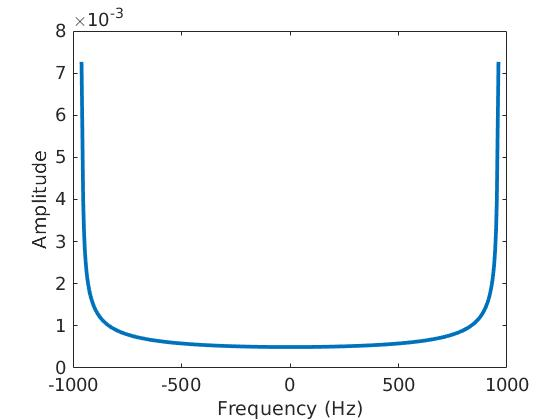
\includegraphics[width=0.45\textwidth]{Sez_Plot.jpg}
    \caption{Example Shaping Spectrum $S_{E_z}$}
    \label{fig:my_label}
\end{figure}

\begin{figure}[h]
    \centering
    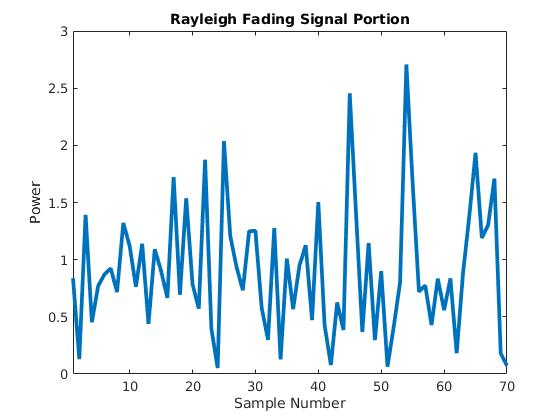
\includegraphics[width=0.45\textwidth]{Example_Rayleigh.jpg}
    \caption{Example Rayleigh Fading Signal}
    \label{fig:my_label}
\end{figure}

\section{Space-Time Block Code Implementation}

Space-time block codes using two antennae are generated from a time domain signal by splitting the signal into its odd and even elements. Let these elements be $s_0$ and $s_1$ representing even and odd respectively. Antenna 0 then alternates between transmitting a symbol from $s_o$ and $-s_1^*$. Antenna 1 transmits symbols from $s_1$ then $s_0^*$. 

The decoding scheme for the code depends on the number of receive antenna present. For a single antenna, the incoming data is again split into even and odd components. Let these be $r_0$ and $r_1$. The received symbols are then determined by $\tilde{s_0} = h_0^*r_0 + h_1r_1^*$ and  $\tilde{s_1} = h_1^*r_0 - h_0r_1^*$ where $h$ represents the known Rayleigh fading channel. The Euclidean distance between each of these symbols and the known BPSK symbols is computed and the closest symbol is selected. After decision making the odd and even components of the signal are combined. Alternatively, the step of computing Euclidean distance can be eliminated by simply looking at the real component of the raw received symbol and checking if it is positive or negative. 

To decode space-time codes when two receive antennae are used, the technique used for the simple single antenna case is extended to include data from both antennae. As previously, the received data is split into odd and even sets, however this now results in 4 sets as there are 2 data sources. Let these be $r_0$, $r_1$, $r_2$, and $r_3$. The received symbols are then determined by  $\tilde{s_0} = h_0^*r_0 + h_1r_1^* + h_2^*r_2 + h_3r_3^*$ and $\tilde{s_0} = h_1^*r_0 + h_0r_1^* + h_3^*r_2 + h_2r_3^*$. The same Euclidean distance decoding scheme as well as data recombination method is used as in the previous case.

\begin{figure}[h]
    \centering
    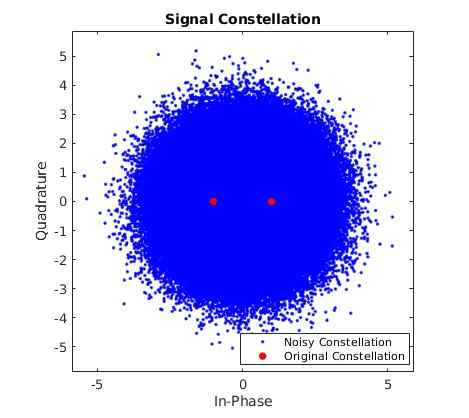
\includegraphics[width=0.45\textwidth]{Sig_Const.jpg}
    \caption{Very Noisy BPSK Signal}
    \label{fig:my_label}
\end{figure}

\begin{figure}[]
    \centering
    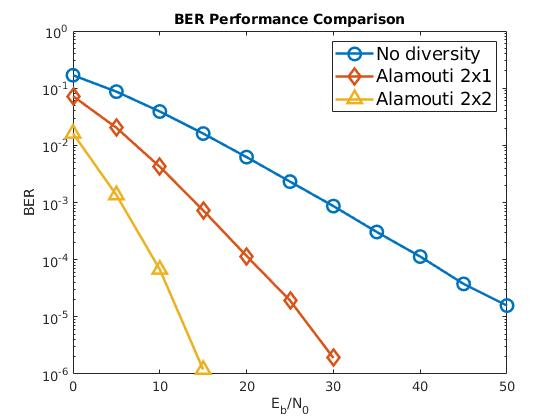
\includegraphics[width=0.45\textwidth]{BER.jpg}
    \caption{Simulated BER Results}
    \label{fig:my_label}
\end{figure}


\section{Sources}
S. M. Alamouti, "A simple transmit diversity technique for wireless communications," in IEEE Journal on Selected Areas in Communications, vol. 16, no. 8, pp. 1451-1458, Oct. 1998. \\
\noindent
T. S. Rappaport, Wireless Communications Principles and Practice, Prentice Hall, 2002. \\
\noindent
J. I. Smith, "A Computer Generated Multipath Fading Simulation for Mobile Radio", IEEE Trans. Vehicular Technology, vol. 24, no. 3, pp. 39-40, Aug. 1975.
 
\end{document}

